\documentclass[a4paper,12pt]{article}
%\usepackage[latin1]{inputenc}
\usepackage[spanish]{babel}
\usepackage{graphicx}
\usepackage{amsmath}
\usepackage{wrapfig}
\setlength{\textheight}{250mm}
\setlength{\textwidth}{165mm}
\setlength{\topmargin}{-15mm}
\setlength{\oddsidemargin}{0pt}
\pagestyle{empty}

\begin{document}

\def\bm#1{{\mbox{\boldmath $#1$}}}
\def\eqdef{\buildrel \rm def \over =}
\def\signo{\mathop{\rm signo}\nolimits}

\mbox{}\vspace*{-20mm}

{\centering
{\small\sc Escuela Técnica Superior de Ingenieros de Caminos, Canales y Puertos (Madrid)}\\*[4mm]
{\Large\bf Método de los Elementos Finitos 23-24}\\*[4mm]
Examen Final - Ejercicio 2. \\*[4mm]
}

% \vspace{4mm}

\noindent
Se considera una lámina cilíndrica de radio medio $R=300$,
longitud $L=600$ y espesor $t=3$, cuyo material es elástico lineal con
propiedades mecánicas $E=300$ y $\nu=0.3$. En los extremos del cilindro hay
dos diafragmas rígidos circulares, y en dos puntos diametralmente
opuestos de la sección transversal media están aplicadas sendas cargas radiales
de compresión de valor $P=1.0$ cada una de ellas. Este es un ejemplo clásico
del análisis de láminas, que en esta práctica se analiza con elementos sólidos
tridimensionales. Para la discretización se tendrán en cuenta las condiciones de
simetría existentes, y se utilizarán discretizaciones de $8 \times 8$ elementos en dirección
meridional y circunferencial y $1$ elemento en el espesor. Las formulaciones a considerar son hexaedros lineales (C3D8), hexaedros cuadráticos (C3D20) y hexaedros lineales con formulación de modos incompatibles (C3D8I).

\vspace{5mm}
\begin{center}
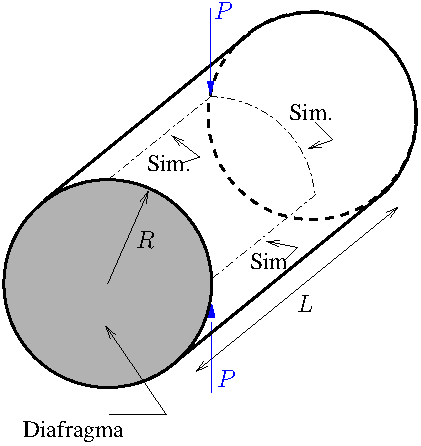
\includegraphics[width=0.50\textwidth]{pinched}
\end{center}
\end{document}
